\documentclass[aspectratio=169,10pt]{beamer}

\usetheme{Boadilla}
\usecolortheme{default}
\usepackage[T1]{fontenc}
\usepackage[utf8]{inputenc}
\usepackage{lmodern}
\usepackage{booktabs}
\usepackage{tabularx}
\usepackage{tikz}
\usetikzlibrary{arrows.meta,positioning,shapes.misc}

\definecolor{TBLNavy}{RGB}{20,35,58}
\definecolor{TBLBlue}{RGB}{40,111,160}
\definecolor{TBLTeal}{RGB}{24,145,137}
\definecolor{TBLLight}{RGB}{239,245,249}
\definecolor{TBLMuted}{RGB}{91,105,120}
\setbeamercolor{structure}{fg=TBLBlue}
\setbeamercolor{title}{fg=white,bg=TBLNavy}
\setbeamercolor{frametitle}{fg=white,bg=TBLNavy}
\setbeamercolor{block title}{fg=white,bg=TBLBlue}
\setbeamercolor{block body}{fg=TBLNavy,bg=TBLLight}
\setbeamercolor{alerted text}{fg=TBLTeal}
\setbeamertemplate{navigation symbols}{}
\setbeamertemplate{footline}{%
  \leavevmode%
  \hbox{%
    \begin{beamercolorbox}[wd=.78\paperwidth,ht=2.6ex,dp=1.1ex,leftskip=1em]{author in head/foot}%
      \color{TBLMuted}\insertshorttitle\hspace{1em}\textbar\hspace{1em}TBL221
    \end{beamercolorbox}%
    \begin{beamercolorbox}[wd=.22\paperwidth,ht=2.6ex,dp=1.1ex,rightskip=1em plus 1fil]{date in head/foot}%
      \color{TBLMuted}\insertframenumber/\inserttotalframenumber
    \end{beamercolorbox}%
  }%
}
\setbeamertemplate{itemize item}{\color{TBLTeal}\small\raise0.2ex\hbox{\scriptsize$\blacktriangleright$}}
\setbeamertemplate{itemize subitem}{\color{TBLBlue}\scriptsize$\bullet$}
\setbeamersize{text margin left=8mm,text margin right=8mm}
\setlength{\parskip}{0.35em}
\setlength{\emergencystretch}{3em}

\title[Linux Resource Monitor]{Linux System Resource Monitoring\\and Graphical Reporting}
\subtitle{A lightweight recorder, durable history, and desktop dashboard}
\author{Yiğit Cemal Öztürk \and Murat Karatekin}
\institute{Kocaeli University \\ Faculty of Technology \\ Department of Information Systems Engineering \\ TBL221 Linux Operating System Usage and Administration}
\date{10 slides \textbullet\ approximately 12 minutes}

\newcommand{\slidepace}[1]{\hfill{\scriptsize\color{TBLMuted}#1}}
\newcommand{\metric}[2]{\begin{beamercolorbox}[rounded=true,sep=0.8em,center,wd=0.30\textwidth]{block body}\textbf{\color{TBLBlue}#1}\\[0.25em]#2\end{beamercolorbox}}

\begin{document}

% 0:30
\begin{frame}[plain]
  \titlepage
  \vspace{-0.7em}
  \begin{center}
    {\small\color{TBLMuted}A practical Linux monitoring system built around standard interfaces and SQLite}
  \end{center}
\end{frame}

% 1:00
\begin{frame}{The goal: turn momentary readings into useful history}
\slidepace{~1:00}
\begin{columns}[T,onlytextwidth]
  \column{0.53\textwidth}
    \begin{block}{The problem}
      A one-time view shows what the machine is doing now, but not how resource use changes over time or when a limit was crossed.
    \end{block}
    \begin{itemize}
      \item Collect system-wide metrics on a configurable schedule.
      \item Keep data collection independent of the graphical session.
      \item Make recent values, trends, and threshold events easy to inspect.
    \end{itemize}
  \column{0.42\textwidth}
    \begin{block}{Project in one sentence}
      A Python recorder samples Linux resources, stores timestamped readings in SQLite, and feeds a read-only PySide6 dashboard.
    \end{block}
    \vspace{0.4em}
    \centering\textbf{Linux-first}\quad\textbullet\quad\textbf{local data}\quad\textbullet\quad\textbf{separate UI}
\end{columns}
\end{frame}

% 1:30
\begin{frame}{A small pipeline keeps collection and presentation separate}
\slidepace{~1:30}
\centering
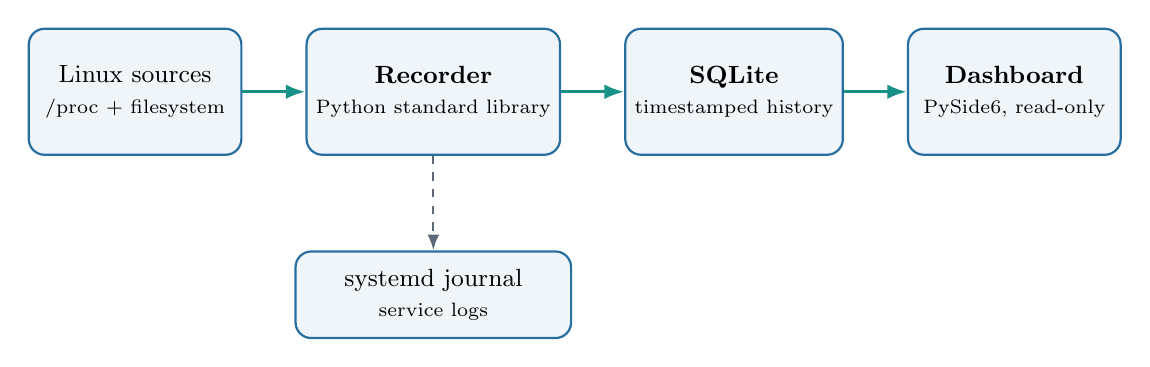
\begin{tikzpicture}[
  node distance=8mm and 8mm,
  unit/.style={draw,rounded corners=2mm,fill=TBLLight,draw=TBLBlue,thick,align=center,minimum width=27mm,minimum height=16mm,font=\small},
  flow/.style={-{Latex[length=2.5mm]},very thick,TBLTeal},
  aux/.style={-{Latex[length=2mm]},thick,TBLMuted,dashed}
]
  \node[unit] (linux) {Linux sources\\\scriptsize /proc + filesystem};
  \node[unit,right=of linux] (recorder) {\textbf{Recorder}\\\scriptsize Python standard library};
  \node[unit,right=of recorder] (db) {\textbf{SQLite}\\\scriptsize timestamped history};
  \node[unit,right=of db] (ui) {\textbf{Dashboard}\\\scriptsize PySide6, read-only};
  \node[unit,below=12mm of recorder,minimum width=35mm,minimum height=11mm] (journal) {systemd journal\\\scriptsize service logs};
  \draw[flow] (linux) -- (recorder);
  \draw[flow] (recorder) -- (db);
  \draw[flow] (db) -- (ui);
  \draw[aux] (recorder) -- (journal);
\end{tikzpicture}
\vspace{1em}
\begin{itemize}
  \item The recorder is the only writer; the GUI opens the database in read-only mode.
  \item The service can continue recording when the dashboard is closed.
  \item SQLite WAL mode supports the intended writer-plus-reader use case.
\end{itemize}

\end{frame}

% 1:20
\begin{frame}{Measurements use native Linux data sources}
\slidepace{~1:20}
\begin{center}
\begin{tabularx}{\textwidth}{@{}>{\raggedright\arraybackslash}p{0.22\textwidth}>{\raggedright\arraybackslash}p{0.25\textwidth}X@{}}
\toprule
\textbf{Metric} & \textbf{Source} & \textbf{How it is represented} \\
\midrule
CPU utilization & \texttt{/proc/stat} & Difference between successive CPU counter samples \\
Memory and swap & \texttt{/proc/meminfo} & Used / total; available memory is preferred \\
Disk usage & Filesystem statistics & Used / total for the configured path \\
Process count & Numeric directories in \texttt{/proc} & Count of visible process entries \\
System load & \texttt{os.getloadavg()} & 1-, 5-, and 15-minute averages \\
\bottomrule
\end{tabularx}
\end{center}
\vspace{0.5em}
\begin{columns}[T,onlytextwidth]
  \column{0.48\textwidth}
    \begin{block}{Sampling behavior}\raggedright
      Default interval: 5 seconds. Scheduling uses a monotonic clock to avoid drift from wall-clock adjustments.
    \end{block}
  \column{0.48\textwidth}
    \begin{block}{Resilient operation}\raggedright
      SIGINT/SIGTERM trigger graceful shutdown; common measurement errors are logged without ending the service loop.
    \end{block}
\end{columns}

\end{frame}

% 1:10
\begin{frame}{SQLite stores both history and threshold events}
\slidepace{~1:10}
\begin{columns}[T,onlytextwidth]
  \column{0.48\textwidth}
    \begin{block}{Readings}
      Each record includes a timestamp, CPU, memory, swap, disk, process count, and three load averages. Capacity values are stored in bytes.
    \end{block}
    \begin{block}{Retention}
      The default policy retains 30 days of measurements; the retention period is configurable.
    \end{block}
  \column{0.48\textwidth}
    \begin{block}{Default alert thresholds}
      \begin{tabular}{@{}lr@{}}
        CPU & 85\% \\
        Memory & 85\% \\
        Disk & 90\% \\
        1-minute load & 8.0 \\
      \end{tabular}
    \end{block}
    \begin{itemize}
      \item Thresholds and cooldown are configurable in TOML.
      \item Alerts are written to SQLite and logged.
      \item Same-metric repeats are suppressed for 300 seconds by default.
    \end{itemize}
\end{columns}
\end{frame}

% 1:20
\begin{frame}{The dashboard turns recent records into an at-a-glance view}
\slidepace{~1:20}
\begin{columns}[T,onlytextwidth]
  \column{0.52\textwidth}
    \begin{block}{Dashboard capabilities}
      \begin{itemize}
        \item Current CPU, memory, disk, and process-count cards.
        \item Time-series charts for CPU, memory, disk, and 1-minute load.
        \item Recent alert table and configurable history window (10--1000 samples).
        \item Manual refresh, automatic 5-second refresh, and CSV export.
      \end{itemize}
    \end{block}
  \column{0.40\textwidth}
    \centering
    {\small\color{TBLMuted}Interface layout (schematic, not a screenshot)}\\[0.5em]
    \resizebox{\linewidth}{!}{%
    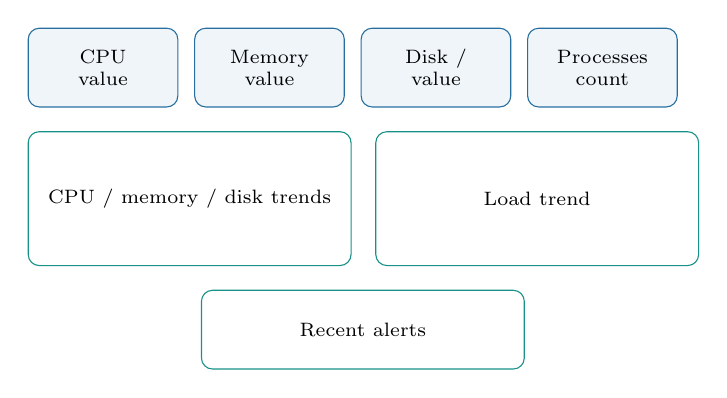
\begin{tikzpicture}[
      card/.style={draw=TBLBlue,rounded corners,fill=TBLLight,minimum width=19mm,minimum height=10mm,align=center,font=\scriptsize},
      chart/.style={draw=TBLTeal,rounded corners,fill=white,minimum width=41mm,minimum height=17mm,align=center,font=\scriptsize}
    ]
      \node[card] (c1) {CPU\\value};
      \node[card,right=2mm of c1] (c2) {Memory\\value};
      \node[card,right=2mm of c2] (c3) {Disk /\\value};
      \node[card,right=2mm of c3] (c4) {Processes\\count};
      \node[chart,below=3mm of c1,xshift=11mm] (g1) {CPU / memory / disk trends};
      \node[chart,right=3mm of g1] (g2) {Load trend};
      \node[chart,below=3mm of g1,xshift=22mm,minimum height=10mm] (alerts) {Recent alerts};
    \end{tikzpicture}%
    }
    \vspace{0.5em}
    {\scriptsize SQLite access is read-only; chart rendering uses Qt painting.}
\end{columns}
\end{frame}

% 1:10
\begin{frame}{Run it locally or install the recorder as a service}
\slidepace{~1:10}
\begin{columns}[T,onlytextwidth]
  \column{0.53\textwidth}
    \begin{block}{Quick local run}
      \scriptsize
      \texttt{python3 tbl221-record/main.py --once}\\
      \texttt{\hspace{1em}--database /tmp/tbl221.db --verbose}\\[0.4em]
      \texttt{python3 -m pip install PySide6}\\
      \texttt{python3 tbl221-graphui/main.py}\\
      \texttt{\hspace{1em}--database /tmp/tbl221.db}
    \end{block}
    Python 3.11+ is required. The recorder itself has no third-party runtime dependency.
  \column{0.42\textwidth}
    \begin{block}{Service and packaging}
      \begin{itemize}
        \item systemd installer, service unit, and manual pages.
        \item Service hardening includes restricted write paths and systemd protections.
        \item Build targets cover Python distributions and Debian/RPM packages.
      \end{itemize}
    \end{block}
    \scriptsize\texttt{sudo python3 tbl221-record/install.py install}
\end{columns}

\end{frame}

% 1:30
\begin{frame}{Validation focuses on the recorder's core behaviors}
\slidepace{~1:30}
\begin{center}
\small
\begin{tabular}{@{}p{0.25\textwidth}p{0.51\textwidth}p{0.14\textwidth}@{}}
\toprule
\textbf{Check} & \textbf{What it covers} & \textbf{Result} \\
\midrule
Unit tests & CPU parsing and delta calculation; memory conversion; SQLite round-trip; alert cooldown & 4/4 passed \\
Compile check & Recorder, GUI, and packaging helper Python sources & Passed \\
\bottomrule
\end{tabular}
\end{center}
\vspace{0.7em}
\begin{block}{Reproduced for this presentation}
  \texttt{make test} completed successfully: compile checks passed and all four unit tests passed.
\end{block}
\begin{alertblock}{Scope of the evidence}
  The unit suite is small and primarily exercises recorder internals. It does not constitute a full GUI interaction or systemd installation test.
\end{alertblock}
\end{frame}

% 1:10
\begin{frame}{Known gaps point to focused next steps}
\slidepace{~1:10}
\begin{columns}[T,onlytextwidth]
  \column{0.48\textwidth}
    \begin{block}{Current limitations}
      \begin{itemize}
        \item Alert cooldown state is in memory and resets after a recorder restart.
        \item GUI warning colors use hardcoded levels, separate from recorder TOML thresholds.
        \item GUI behavior has only a basic startup smoke check, not detailed widget tests.
      \end{itemize}
    \end{block}
  \column{0.48\textwidth}
    \begin{block}{Practical improvements}
      \begin{itemize}
        \item Persist cooldown state if restart continuity is required.
        \item Share threshold definitions with the dashboard.
        \item Add GUI and configuration tests, including failure-path coverage.
      \end{itemize}
    \end{block}
\end{columns}
\vspace{0.5em}
\centering\small\color{TBLMuted}These are maintenance opportunities, not claims that the current core monitoring path is unavailable.
\end{frame}

% 1:00
\begin{frame}[plain]
\vfill
\centering
{\Huge\color{TBLNavy}\textbf{Collect. Preserve. Understand.}}\\[0.7em]
{\large Linux metrics become actionable when their history and threshold events are easy to inspect.}\\[1.5em]
{\Large\color{TBLTeal}Questions?}\\[2em]
{\small\color{TBLMuted}Source: project README, report, and implementation. \\
Linux metrics: \texttt{/proc}; persistence: SQLite; GUI: PySide6.}
\vfill
\end{frame}

\end{document}
